\section{Behaviors}
\label{sec:Behaviors}
% Owner: Jani
% Reviewed:
%
The addressed solution provides in its default setting already several behaviors for merchants as well as the consumers. In this chapter, we will outline and describe the underlying behaviors which are currently available.

\subsection{Merchant}
\label{sec:Behaviors_Merchants}
% Owner: Johanna, Jani
% Reviewed:
%
The merchant-component has one main task: The calculation of a price for a given product. This can either be a new product, purchased from the producer, or an existing product, that is already on the marketplace as an offer. This calculation has to take the trade-off between maximizing the probability to sell a product and maximizing the own profit into account. \\

To allow an easy start, the platform already offers a set of five rule-based strategies and one data-driven approach, that implements a pricing strategy based on logistic regression \citep{hosmer2013applied}.

%
\subsubsection{Rule-based merchants}
%
The simple, rule-based behaviors include ``Be the \textit{n}th-cheapest'', ``Fixed pricing'', ``Randomly be the 1st, 2nd or 3rd cheapest'' and the ``Gas Station strategy'' (also called ``Two Bound'' in our system). The ``Two Bound'' strategy sets a minimum and maximum profit margin that can be added to the product's purchase price. The strategy keeps lowering the price to be the cheapest until the minimum bound is reached - then the algorithm sets the price for this product to the maximum profit margin (see fig. \ref{fig:price_graphs_v2}). \\

%
\begin{figure}[h]
    \centering
    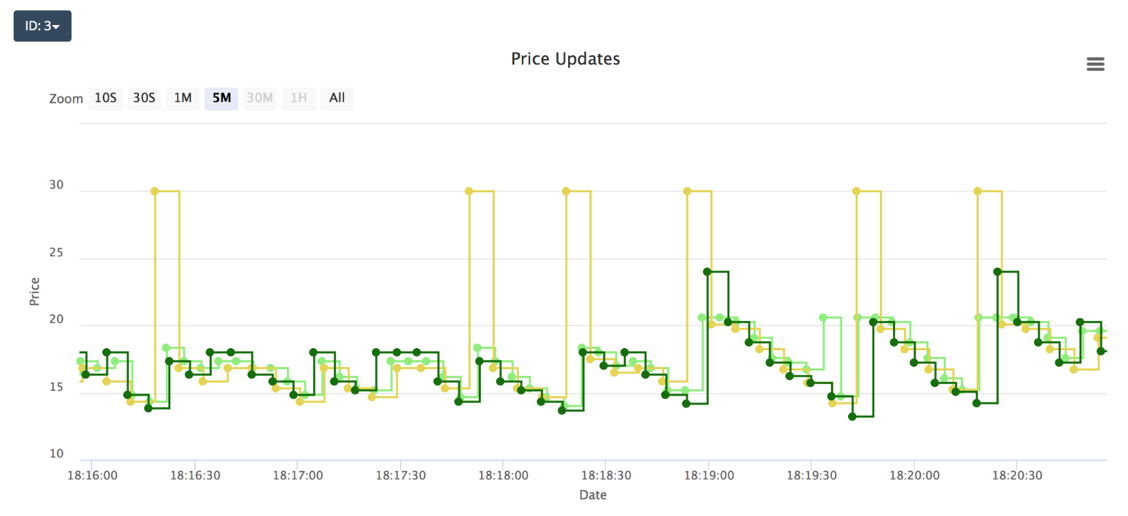
\includegraphics[width=0.5\textwidth]{images/price_graphs_v2.png}
    \caption{Price Graphs}
    \label{fig:price_graphs_v2}
\end{figure}
%

%
\subsubsection{Data-driven merchant}
%
The data-driven behavior follows a pricing strategy aimed at maximizing the expected profit. To do so, a logistic regression model is trained, based on features such as the distance to the cheapest competitor, the price- and quality-rank, the number of competitors or the average price of the product on the marketplace. The data used to learn this model are past market situations in which the merchant sold his own product, i.e. the dependent variable representing whether a product was sold or not is true. The merchant can only use his own sales data to train the model - the access to sales data of other merchants is restricted by the system, just as it is the case in real-life marketplaces. As a result, the logistic regression model outputs the probability with which a product is sold, given a certain market situation and price for that product. To maximize the expected profit, this merchant comes up with a set of possible prices for a product, calculates the selling probability in the current situation, multiplies this probability with the corresponding price and as a result gets the expected profit for each possible price. \\

All of these behaviors have certain base settings that further determine the behaviors and that can be adjusted during run time. These are inter alia the number of starting products the merchant buys from the producer or a minimum profit margin that this merchant will never undercut.

Additionally, an SdK in Python was implemented to facilitate an easy on-boarding and extension of the platform by adding custom merchants.

\subsection{Consumer}
\label{sec:Behaviors_Consumer}
% Owner: Jani
% Reviewed: Johanna
%

A consumer-component is included in the deployment provideing several buying behaviors which can be chosen, weighted, and reconfigured on-the-fly. Those behaviors range from very subtle approaches like buying the $n$th-cheapest, first, most expensive or simply random offers on the marketplace up to more sophisticated methods trying to imitate more complex consumer situations. A sigmoid distribution with twice of the producer price as mean (see fig. \ref{fig:sigmoid_distribution}) is available through the default settings as well as a data-driven ``logit''-behavior.

%
%\begin{figure}[h]
%    \centering
%    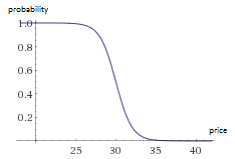
\includegraphics[width=0.25\textwidth]{images/sigmoid.png}
%    \caption{Sigmoid distribution as consumer behavior}
%    \label{fig:sigmoid_distribution}
%\end{figure}
%

The logit-behavior implements a logistic regression with feature scaling and calculates for each offer the buying probability based on the feature coefficients provided in the behavior settings. Based on this buying probability for each offer, the consumer will actually choose an offer to buy. In this way, potential consumer behavior can be learned on real world data and imitated in the simulation solution.

The default settings for the logit-behavior holds coefficients which were extracted from a real-world use case provided by a big book retail company. For deeper insights in the concepts of logistic regression, the reader is kindly referred to \citet{hosmer2013applied}'s elaboration.

% Johanna: Würde ich ganz rauslassen, Logistic Regression zu erklären ist nicht Thema oder Aufgabe vom Paper. Der Verweis oben reicht mMn.
%\subsection{Logistic Regression}
%\label{sec:Logistic_Regression}
% Owner: Jani
% Reviewed:
%
%Logistic regression is a regression model where the dependent variable -- in our case the selling of an offer -- is categorical. This categorization outcome must be discrete and should be dichotomous in nature simply expressed by a Boolean whether a purchase happened or not. To determine this, this behavior consumes features and their coefficients can be altered at runtime and will then be applied to the next calculation iteration taking place. The describing hashmap of features and their coefficients contains only available features which are already implemented. Otherwise they will be ignored.
